%%%%%%%%%%%%%%%%%%%%%%%%%%%%%%%%%%%%%%%
% Original author:
% Meet Bhatnagar
%
% Original repository:
% https://github.com/MeetDarkPow/meet-Res
%%%%%%%%%%%%%%%%%%%%%%%%%%%%%%%%%%%%%%

\documentclass[]{meetresume-class}


\begin{document}
	
	%%%%%%%%%%%%%%%%%%%%%%%%%%%%%%%%%%%%%%
	%
	%     COLUMN ONE
	%
	%%%%%%%%%%%%%%%%%%%%%%%%%%%%%%%%%%%%%%
	
	\begin{minipage}[t]{0.33\textwidth} 
		\begin{large}
			\headername{Meet Bhatnagar}\\
		\end{large}
		Third Year (B.Tech)\\
		Computer Science $\&$ Engineering\\ 
		at VIT Vellore \\ 
		CGPA : 8.28 till \nth{5} Semester 
		
		%%%%%%%%%%%%%%%%%%%%%%%%%%%%%%%%%%%%%%
		%     LINKS
		%%%%%%%%%%%%%%%%%%%%%%%%%%%%%%%%%%%%%%
		\section{Links} 
		\noindent\rule{5cm}{0.6pt}
		
		\href{https://github.com/MeetDarkPow}{\custombold{GitHub}}:\\
		https://github.com/MeetDarkPow \\
		\href{https://www.linkedin.com/in/meet-bhatnagar-a41842181/}{\custombold{LinkedIn}}:\\
		www.linkedin.com/in/meet-bhatnagar
		\sectionsep
		%%%%%%%%%%%%%%%%%%%%%%%%%%%%%%%%%%%%%%
		%     SKILLS
		%%%%%%%%%%%%%%%%%%%%%%%%%%%%%%%%%%%%%%
		\section{Skills}
		\noindent\rule{5cm}{0.6pt}
	
		%\subsection{OS}
		%Windows
		%\vspace{6pt}
		
		\subsection{Languages}
		Proficient: C/C++, R Programming
		%Familiar: HTML, CSS, JavaScript
		\vspace{6pt}
		
		\subsection{Data Science}
		Data Visualization, Data Analysis,\\
		Data Mining, Data Cleaning
		\vspace{6pt}
		
		\subsection{Databases}
		MySQL%, PostgreSQL
		\vspace{6pt}
		
		\subsection{Others}
		R Markdown, GitHub Desktop, RStudio,\\
		MiKTeX, MATLAB
		\sectionsep
		%%%%%%%%%%%%%%%%%%%%%%%%%%%%%%%%%%%%%%
		%     COURSEWORK
		%%%%%%%%%%%%%%%%%%%%%%%%%%%%%%%%%%%%%%
		\section{Coursework}
		\noindent\rule{5cm}{0.6pt}
		
		Data Structures\\
		Algorithm\\
		%System Design\\
		%Computer Networks\\
		Operating Systems\\
		DBMS\\
		Data Science
		\sectionsep
		%%%%%%%%%%%%%%%%%%%%%%%%%%%%%%%%%%%%%%
		%     EDUCATION
		%%%%%%%%%%%%%%%%%%%%%%%%%%%%%%%%%%%%%%
		\section{Education} 
		\noindent\rule{5cm}{0.6pt}\\
		\datecolor{2018-Present}
		\subsection{B.Tech. - CSE}
		VIT Vellore, Tamil Nadu \\
		CGPA : 8.28/10\\
		\vspace{8pt}
		\datecolor{2016-2017}
		\subsection{CBSE - Intermediate}
		RKVM, Gwalior (M.P.)\\
		Percentage : 82.2\%\\
		\vspace{8pt}
		\datecolor{2014-2015}
		\subsection{CBSE - High School}
		Dewan Public School, Meerut (U.P.)\\
		CGPA : 10/10
		\sectionsep
		%%%%%%%%%%%%%%%%%%%%%%%%%%%%%%%%%%%%%%
		%     CERTIFICATES
		%%%%%%%%%%%%%%%%%%%%%%%%%%%%%%%%%%%%%%
		\section{Certificates}
		\noindent\rule{5cm}{0.6pt}
		
		\href{coursera.org/verify/professional-cert/N792SQ9DZJJR}{Google Data Analytics Professional Certificate (2021)}\\
		\href{https://coursera.org/share/3dbc74a447f9ca4efc319aefd14efa33}{Johns Hopkins University - Data Science Specialization (2020/21)}\\
		\href{https://coursera.org/share/34576e12fe5880c5e3382c8a91b56564}{University of Pennsylvania - Positive Psychology: Visionary Science (2021)}\\
		
	\end{minipage} 
	\hfill
	%%%%%%%%%%%%%%%%%%%%%%%%%%%%%%%%%%%%%%
	%
	%     COLUMN TWO
	%
	%%%%%%%%%%%%%%%%%%%%%%%%%%%%%%%%%%%%%%
	\begin{minipage}[t]{0.66\textwidth} 
		% \descript{BS in Computer ence}
		\hspace*{0pt}\hfill    \\
		\hspace*{0pt}\hfill 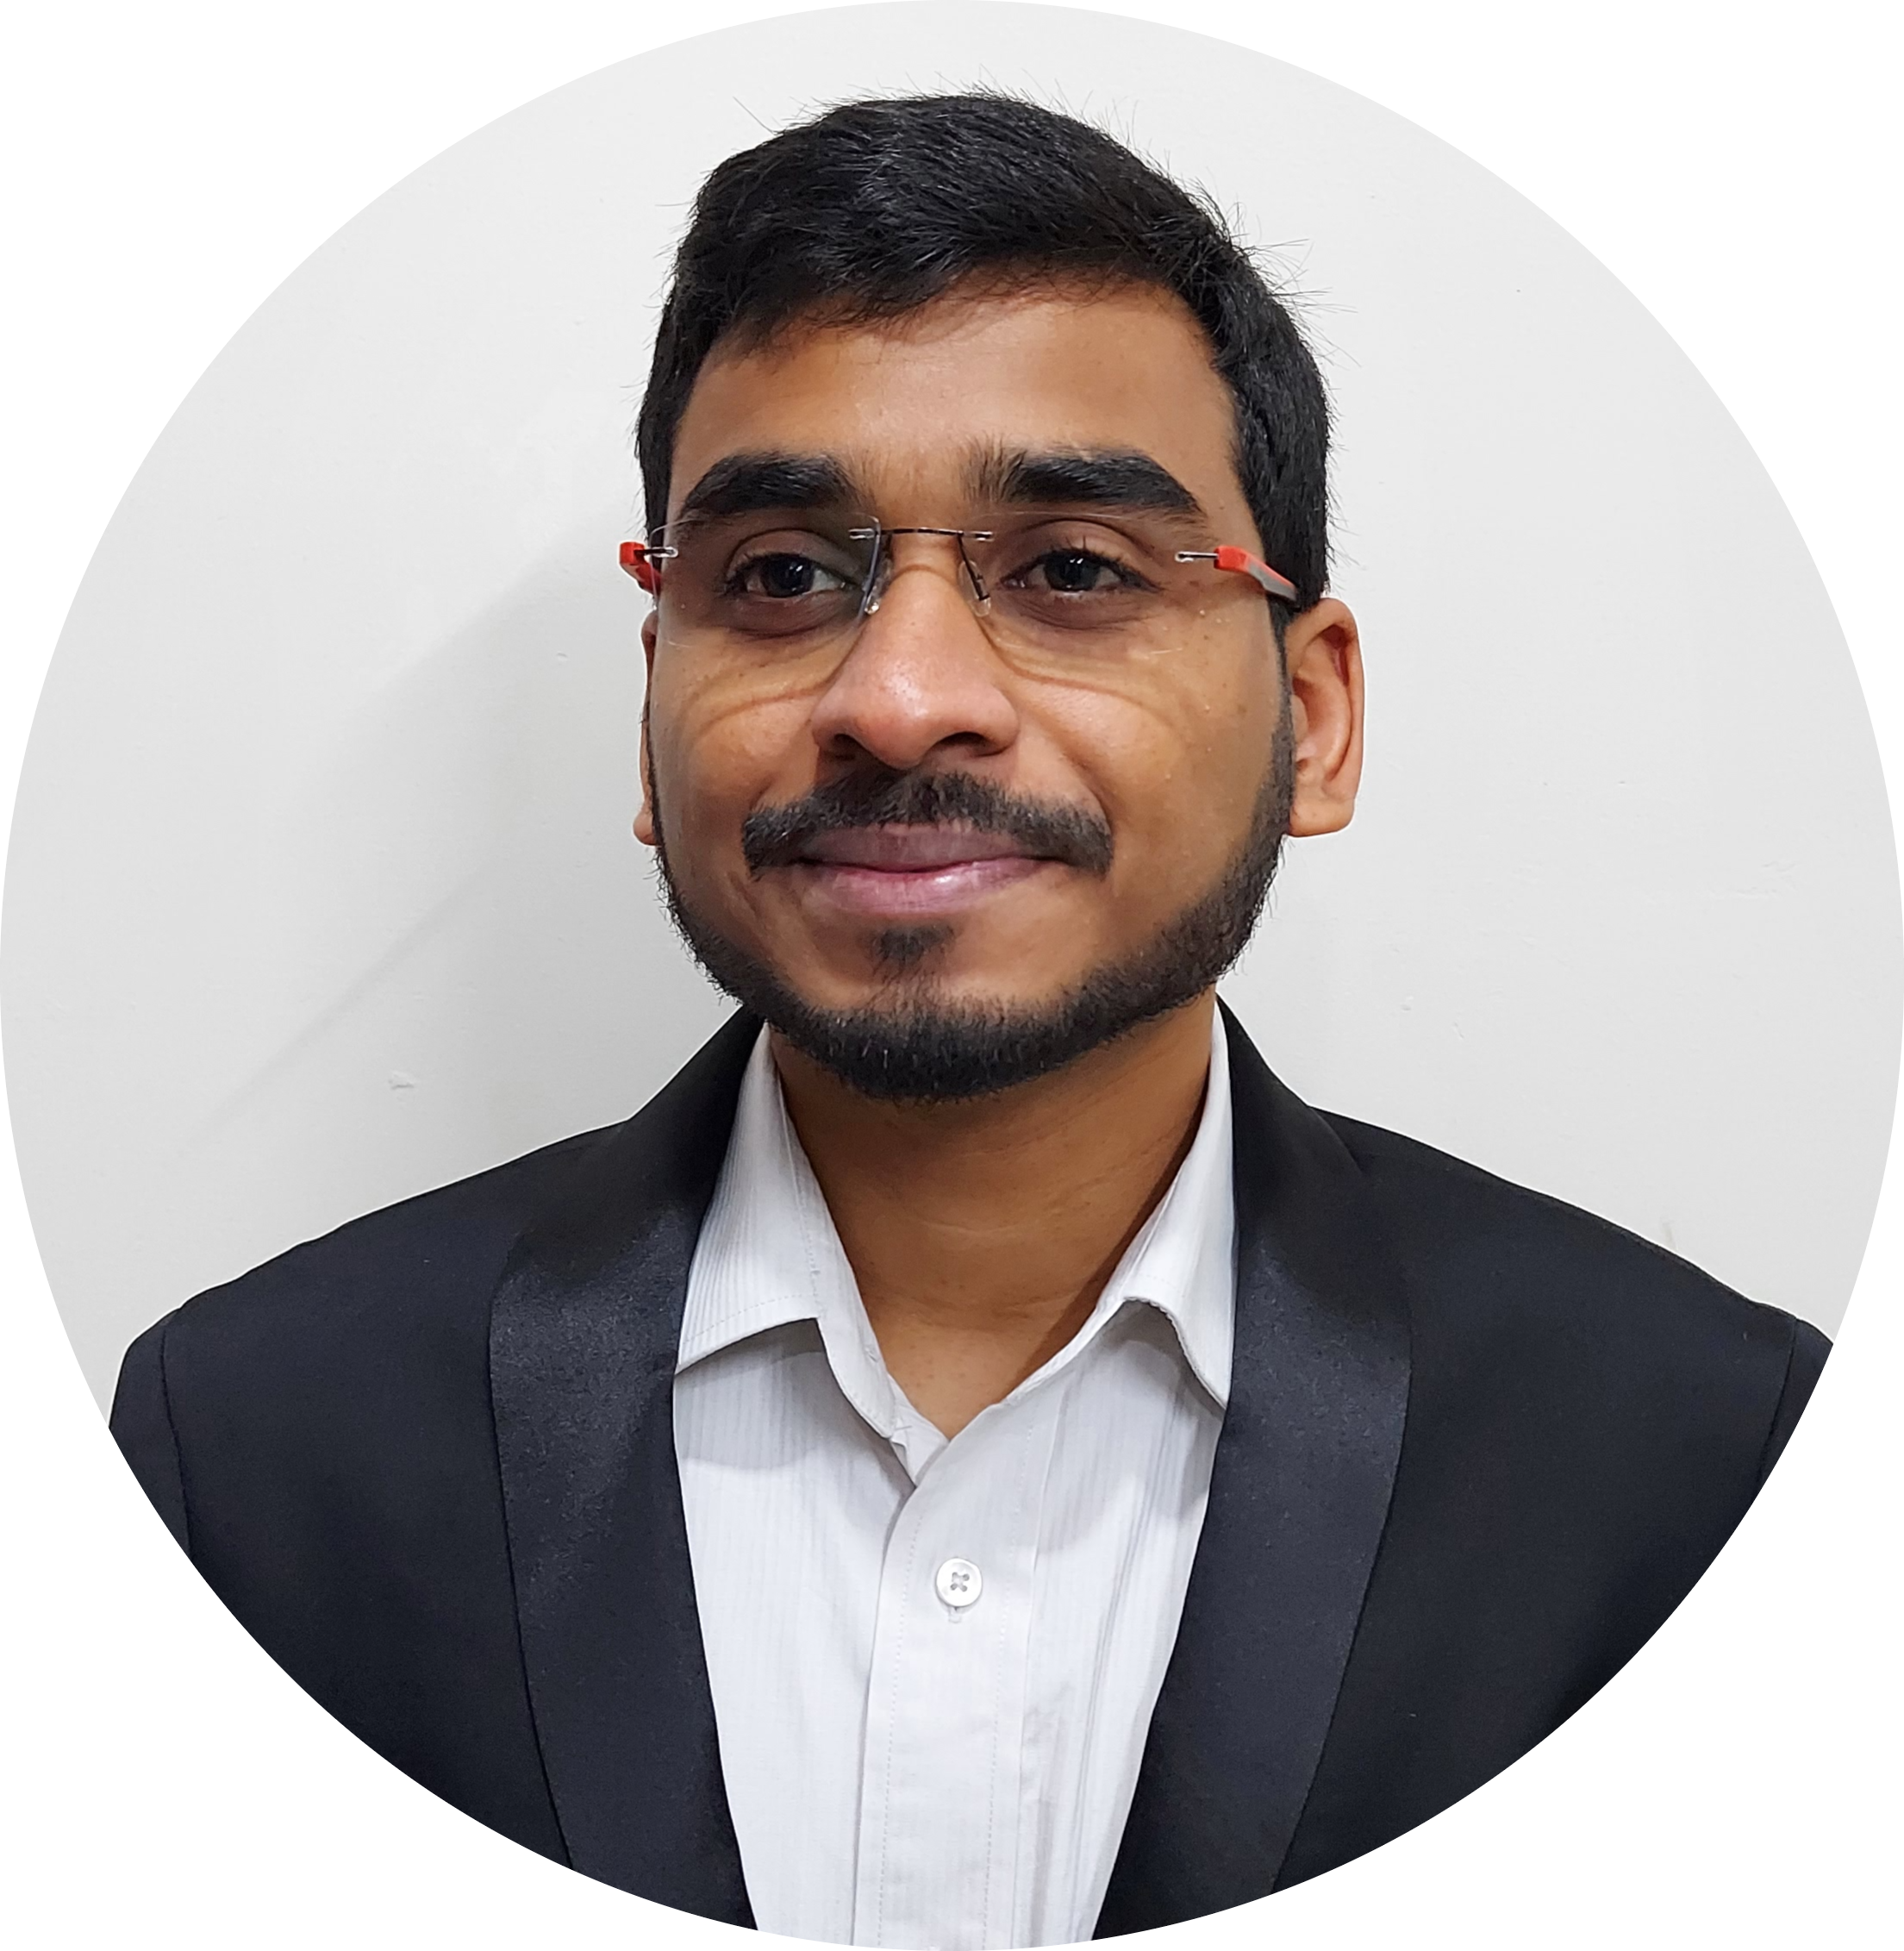
\includegraphics[width=1.8cm, height=1.8cm]{Profile_pic.png}\\
		\hspace*{0pt}\hfill Mobile : +91-6397356028 \\
		\hspace*{0pt}\hfill Email : \textbf{\href{mailto:meet1708@gmail.com}{meet1708@gmail.com}}

		%%%%%%%%%%%%%%%%%%%%%%%%%%%%%%%%%%%%%%
		%     EXPERIENCE
		%%%%%%%%%%%%%%%%%%%%%%%%%%%%%%%%%%%%%%
		\section{Experience}
		\noindent\rule{12.5cm}{0.4pt}
		\datecolor{MAY-Now, 2021} \runsubsection{\href{https://summerofcode.withgoogle.com/projects/\#5835435529469952}{RCE Explorer, Google Summer of Code}}
		\descript{Developer}
		\noindent
		\hspace{5em}%
		\begin{minipage}{0.85\textwidth\vspace{2pt}}
			 Building the framework for monitoring the popularity of R-related events, interests of Global R Community over time. Track, log and visualize R conference/events tweets in a central flexdashboard. Setup pipelines using CI/CD to facilitate the extract, transform and load of related data daily.
		\end{minipage}
		\descriptright{RStudio, leaflet map, Twitter API, StackExchange API, Plotly.js, crosstalk}
		\sectionsep
		\hspace*{0pt}\hfill  \\
		
		\datecolor{MAY-JULY, 2019} \runsubsection{\href{https://github.com/MeetDarkPow/Rainfall-Data-Analysis-India-}{R-FLOSS, FOSSEE IIT Bombay}}
		\descript{Data Analyst Intern}
		\noindent
		\hspace{5em}%
		\begin{minipage}{0.85\textwidth\vspace{2pt}}
			Analyzed 111 years rainfall data of 596 districts of India provided by IMD, Govt. of India. Steps: Data cleaning-Segregation, Data Analysis-Visualization. Analysis, visualizations and predictions were projected on dashboard created via RShiny on RCloud platform.
		\end{minipage}
		\descriptright{RStudio, RMarkdown, RShiny, RCloud, QGIS Mapping}
		\sectionsep
		
		%%%%%%%%%%%%%%%%%%%%%%%%%%%%%%%%%%%%%%
		%     Open Source Contribution
		%%%%%%%%%%%%%%%%%%%%%%%%%%%%%%%%%%%%%%
		\section{Open Source Contributed Projects \& Conferences} 
		\noindent\rule{12.5cm}{0.4pt}
		\datecolor{JULY, 2021} \runsubsection{useR! 2021 - The R User International Conference}
		\descript{}
		\noindent
		\hspace{5em}%
		\begin{minipage}{0.85\textwidth\vspace{2pt}}
			Extracting statistics for R-bloggers website. Analysis on the different types of blogs posted on R-bloggers.
		\end{minipage}
		\sectionsep
		
		\datecolor{2020-Now} \runsubsection{\href{https://github.com/MeetDarkPow/R-Community-Analysis}{R Community Explorer - Google Summer of Code}}
		\descript{}
		\noindent
		\hspace{5em}%
		\begin{minipage}{0.85\textwidth\vspace{2pt}}
			\custombold{2020} - Implementing new functionalities such as CRAN Exploration, CRAN Task Views, Twitter Exploration (\#rstats tweets), GitHub \\Exploration of R repositories.\\
			\custombold{2021} - Presently working on flexdashboard for the project.
		\end{minipage}
		\sectionsep
		
		\datecolor{JULY, 2020} \runsubsection{\href{https://www.youtube.com/watch?v=7F7iQdcV8RY&t=2s&ab_channel=RConsortium}{useR! 2020 - The R User International Conference}}
		\descript{}
		\noindent
		\hspace{5em}%
		\begin{minipage}{0.85\textwidth\vspace{2pt}}
			Data-Driven Exploration of the global R Community. Statistical data analysis for
			CRAN and BioConductor packages, R GitHub Repositories, Q\&A of R related
			posts on Stack Overflow.
		\end{minipage}
		\sectionsep
		
		\datecolor{MAY, 2019} \runsubsection{R TBC Team, IIT Bombay}
		\descript{Reviewer}
		\noindent
		\hspace{5em}%
		\begin{minipage}{0.85\textwidth\vspace{2pt}}
			Reviewed R codes for solved examples of textbooks under TBC \\Project. 
		\end{minipage}
		\sectionsep
		%%%%%%%%%%%%%%%%%%%%%%%%%%%%%%%%%%%%%%
		%     PUBLICATION
		%%%%%%%%%%%%%%%%%%%%%%%%%%%%%%%%%%%%%%
		\section{Publication} 
		\noindent\rule{12.5cm}{0.4pt}
		\datecolor{JUNE, 2020} \runsubsection{\href{https://r.fossee.in/textbook-companion/textbook-run}{Textbook Companion Project}}
		\descript{Author R Codes}
		\noindent
		\hspace{5em}%
		\begin{minipage}{0.85\textwidth\vspace{2pt}}
			Title : Fundamentals of Mathematical Statistics\\
			R code book published under Textbook Companion Project funded
			from the National Mission on Education through ICT.
		\end{minipage}
		%%%%%%%%%%%%%%%%%%%%%%%%%%%%%%%%%%%%%%
		%     SIDE PROJECT
		%%%%%%%%%%%%%%%%%%%%%%%%%%%%%%%%%%%%%%
		\section{Side Project}
		\noindent\rule{12.5cm}{0.4pt}
		\datecolor{JAN, 2019} \runsubsection{Vehicle Number Plate Identification}
		\descript{MATLAB}
		\noindent
		\hspace{5em}%
		\begin{minipage}{0.85\textwidth\vspace{5pt}}
			To recognize the vehicle number plate using MATLAB. An upgraded and
			efficient approach is recognized with high detection rate based on image
			processing and edge detection.
		\end{minipage}
	\end{minipage} 
\end{document}  \documentclass[]{article}